\documentclass[12pt]{article}

\usepackage[giveninits=true]{biblatex}
\usepackage{amsthm, amssymb, amsfonts, amsmath, geometry, enumerate}
\usepackage{url}
\usepackage[]{graphicx}
\usepackage[font=small,labelfont=bf]{caption}
%\geometry{left=1in,right=1in,top=.5in,bottom=1in,headheight=4pt,headsep=0.3in}

\newtheorem{lemma}{Lemma}
\newtheorem{theorem}{Theorem}

\newcommand{\x}{\mathbf{x}}
\newcommand{\X}{\mathbf{X}}
\newcommand{\y}{\mathbf{y}}
\newcommand{\z}{\mathbf{z}}
\renewcommand{\c}{\mathbf{c}}
\newcommand{\C}{\mathcal{C}}
\newcommand{\I}{\mathcal{I}}
\renewcommand{\S}{\mathcal{S}}

\title{Seeding in \texttt{k-means} Clustering}
\author{Masum Billal\\Dhaka, Bangladesh\\\url{billalmasum93@gmail.com}}

\addbibresource{ref.bib}

\newcommand{\scale}{.33}

\begin{document}
	%\maketitle
		\begin{abstract}%
			In machine learning or data mining in general, clustering is one of the most popular methods to extract valuable insights into the data. It becomes even more important when the data is high dimensional that can provide information regarding user behavior or underlying structure or affinity towards a certain direction. KMeans is a popular clustering algorithm that aims to solve the clustering problem by reducing the sum of minimum squared distances from data points to the centers. It is well established by now that seeding centers is better than choosing centers uniformly. In this paper, we first express our concerns about the results presented in k-means++ paper. Then we suggest an improvement, discuss various types of seeding methods and compare their performances. We also establish an upper bound on the inertia function associated with kmeans clustering. The author does not claim any originality regarding the improvement because the author found out later that another paper already considered the improvement suggested in this paper and that {kmeans++} is essentially the same idea. Nonetheless, the paper also serves as an updated survey on the comparison of seeding methods.
		\end{abstract}

		%\begin{keywords}
		%	clustering, \texttt{k-means}, seeding centers, inertia optimization, \texttt{k-means++}
		%\end{keywords}
	\section{Introduction}
	Widely regarded as the most popular clustering techniques, \texttt{k-means} remains a humble interesting topic in machine learning as well as computational geometry. Clustering is still an active field of research as there are a lot of recent developments in this area including some ideas that involve deep learning. This is so primarily because of how useful clustering is in both research and professional areas. For example, companies regularly use clustering to identify their most valuable users (or vice-versa). There have even been cases where some unstructured data have been first clustered and then the corresponding labels have been used to train machine learning models. Roughly the problem of clustering from the point of view of KMeans is: given a set of points $\X$ in $\mathbb{R}^d$. Find a set of centers $\mathcal{C}$ such that the function \textit{inertia}
		\begin{align*}
			\mathcal{I} & = \sum_{\x\in\X}\min_{\c\in\C}(\|\c-\x\|^2)
		\end{align*}
	is minimum where $\|\cdot\|$ is the $L_2$ norm\footnote{$\|c-x\|$ or $L_2$ norm of $\c-\x$ is the distance between the center $\c$ and point $\x$ or the magnitude of the vector $\c-\x$.}.

	Default \texttt{k-means} algorithm starts with random centers and then converge based on minimum distances of the centers from the data points. New centers are calculated based on the centroid. This is known as Lloyd's algorithm \textcite{lloyd_1982}. We repeat this process until no more change is possible. Lloyd's method was published much later. \textcite{forgy_1965} essentially publishes Llyod's method before Lloyd so sometimes we even call it Lloyd-Forgy algorithm. \textcite{Bradley_Fayyad_1998,ostrovsky_rabani_schulman_swamy_2012} and \textcite{arthur_vassilvitskii_2007} take it one step further by choosing the initial centers with a probability. We intend to introduce other ways of initialization and compare their performances in terms of inertia, convergence speed and CPU time taken.

	First, we will discuss some benchmarks for most of the well established algorithms in clustering. Then we discuss a sensitive issue regarding \texttt{k-means++} algorithm. Then we discuss the initialization methods used to compare the performance of clustering. We also prove a theorem that provides an upper bound for the inertia when \texttt{k-means} is done using seeded centers. Finally, we show experimental results for both our argument regarding \texttt{k-means++} and performance of initialization methods. For experimental results, we assumed that an algorithm converges only when the centers do not change anymore, that is, the algorithm absolutely stops changing centers altogether. There are some available techniques of stopping \texttt{k-means} algorithms but we chose not to use any of them as they might produce unreliable results.
	\section{A Brief Comparison  of Synthetic Data}
	There has been multiple surveys and a lot of work on \texttt{k-means} in the literature. For our context, probably the most relevant work is done in \textcite{celebi_kingravi_vela_2013}. However, most of the algorithms used in that paper are practically not very useful. The same was also noted by the authors themselves. They concluded that \texttt{k-means++} and its greedy version work better than most. They also mention that probabilistic algorithms perform better than deterministic ones. Therefore, our primary focus has been on non-deterministic algorithms in this paper. We take this chance to introduce the not so popular algorithm \textcite{ostrovsky_rabani_schulman_swamy_2012} (\texttt{ORSS}). \texttt{ORSS} was not considered in their experiments. As we will show, \texttt{ORSS} is actually a very relevant topic in this regard. Note that we do not  consider Gaussian Mixture Model for the experiment because it has been noted to be significantly slow for practical purposes, see \textcite{Patel_Kushwaha_2020} for a detailed discussion.

	We would like to point out that to our knowledge no surveys were done after removing linear dependency prior to running the experiments. This is a very important step if we are to get a meaningful clustering out of \texttt{k-means} algorithm. We can achieve this using some known algorithm such as \textbf{principle component analysis} (PCA, see \textcite{pearson_1901}, \textcite{hotelling_1933}) . We opted for PCA in this paper. PCA decomposes the existing data points into orthogonal\footnote{It is well known that orthogonal vectors are linearly independent.} ones. If we use PCA before running a clustering algorithm, we can redefine the variables into linearly independent ones. For our experiment, we have used PCA on every data set before running cluster algorithm. However, we did not reduce dimensions in order to preserve the originality of the data set. We only used PCA for removing linear dependency among variables. We strongly believe this strengthens our result over other available results.

	As a refresher we will mention some well known algorithms and compare their performances for practical purposes\footnote{The code used for this experiment is based on scikit-learn library and the code is a modified form of \url{https://scikit-learn.org/stable/auto_examples/cluster/plot_cluster_comparison.html#sphx-glr-auto-examples-cluster-plot-cluster-comparison-py}}. Affinity Propagation by \textcite{Frey_Dueck_2007} discusses a similarity based clustering method but as we will show later, it is very slow and does not scale. But more importantly, the data points do not necessarily always converge as noted in this experiment. There are also hierarchical algorithms such as DBSCAN by \textcite{Ester_Kriegel_Sander_Xu_1996}, HDBSCAN by \textcite{Campello_Moulavi_Sander_2013}, and improvements on DBSCAN and HDBSCAN by \textcite{McInnes_Healy_2017}. OPTICS by \textcite{Ankerst_Breunig_Kriegel_Sander_1999} is a generalization of DBSCAN which aims to build some sort of reachability graph to understand the inner structure of the data points. But for large datasets, similar results can be obtained using HDBSCAN so we do not use OPTICS. \textcite{Comaniciu_Meer_2002} is a robust technique that tries to show convergence of underlying density function and performs relatively well but not as good as KMeans. A comparatively efficient version of \textcite{Yu_Shi_2003} by \textcite{Damle_Minden_Ying_2018} discusses a spectral clustering based on Eigen decomposition although it struggles to scale. There is also BIRCH by \textcite{Zhang_Ramakrishnan_Livny_1996} which is based on a tree called cluster feature tree. However, it also struggles with high dimensional data, specially if the dimension is over $20$.

	The summary of the following results is that, considering all factors, KMeans is the only realistic solution clustering any kind of data. It also offers the extra benefit for us to choose the number of clusters and that is also sometimes important. The practical implication is that some methods e.g. Affine Propagation

	\begin{center}
		\begin{minipage}{\linewidth}
			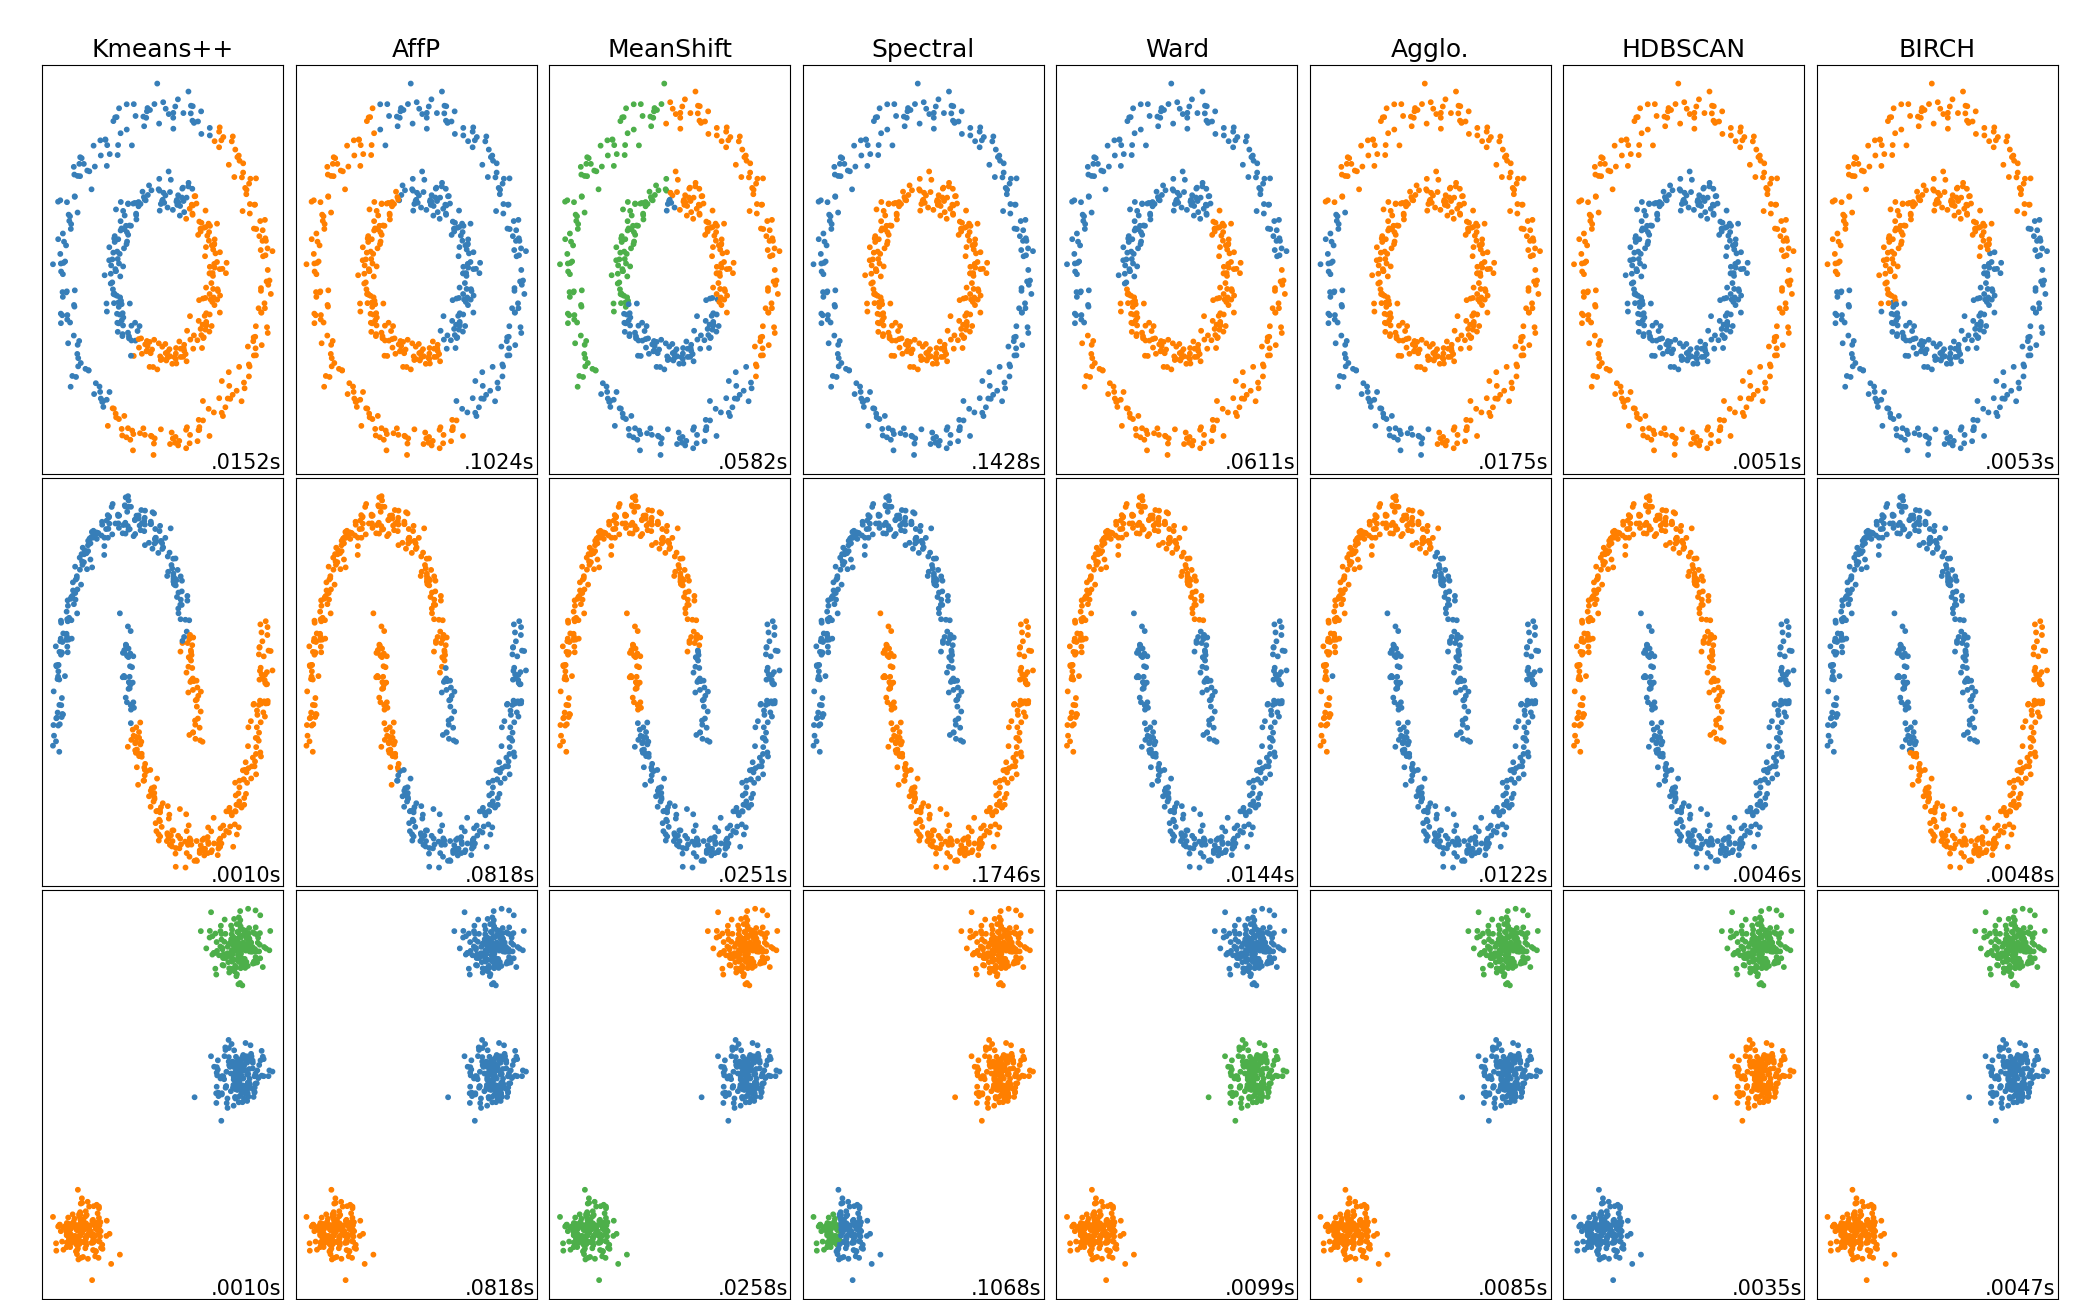
\includegraphics[width=\linewidth]{../clustering_result_500}
			\captionof{figure}{Time taken for 500 points}
		\end{minipage}
	\end{center}

	\begin{center}
		\begin{minipage}{.9\linewidth}
			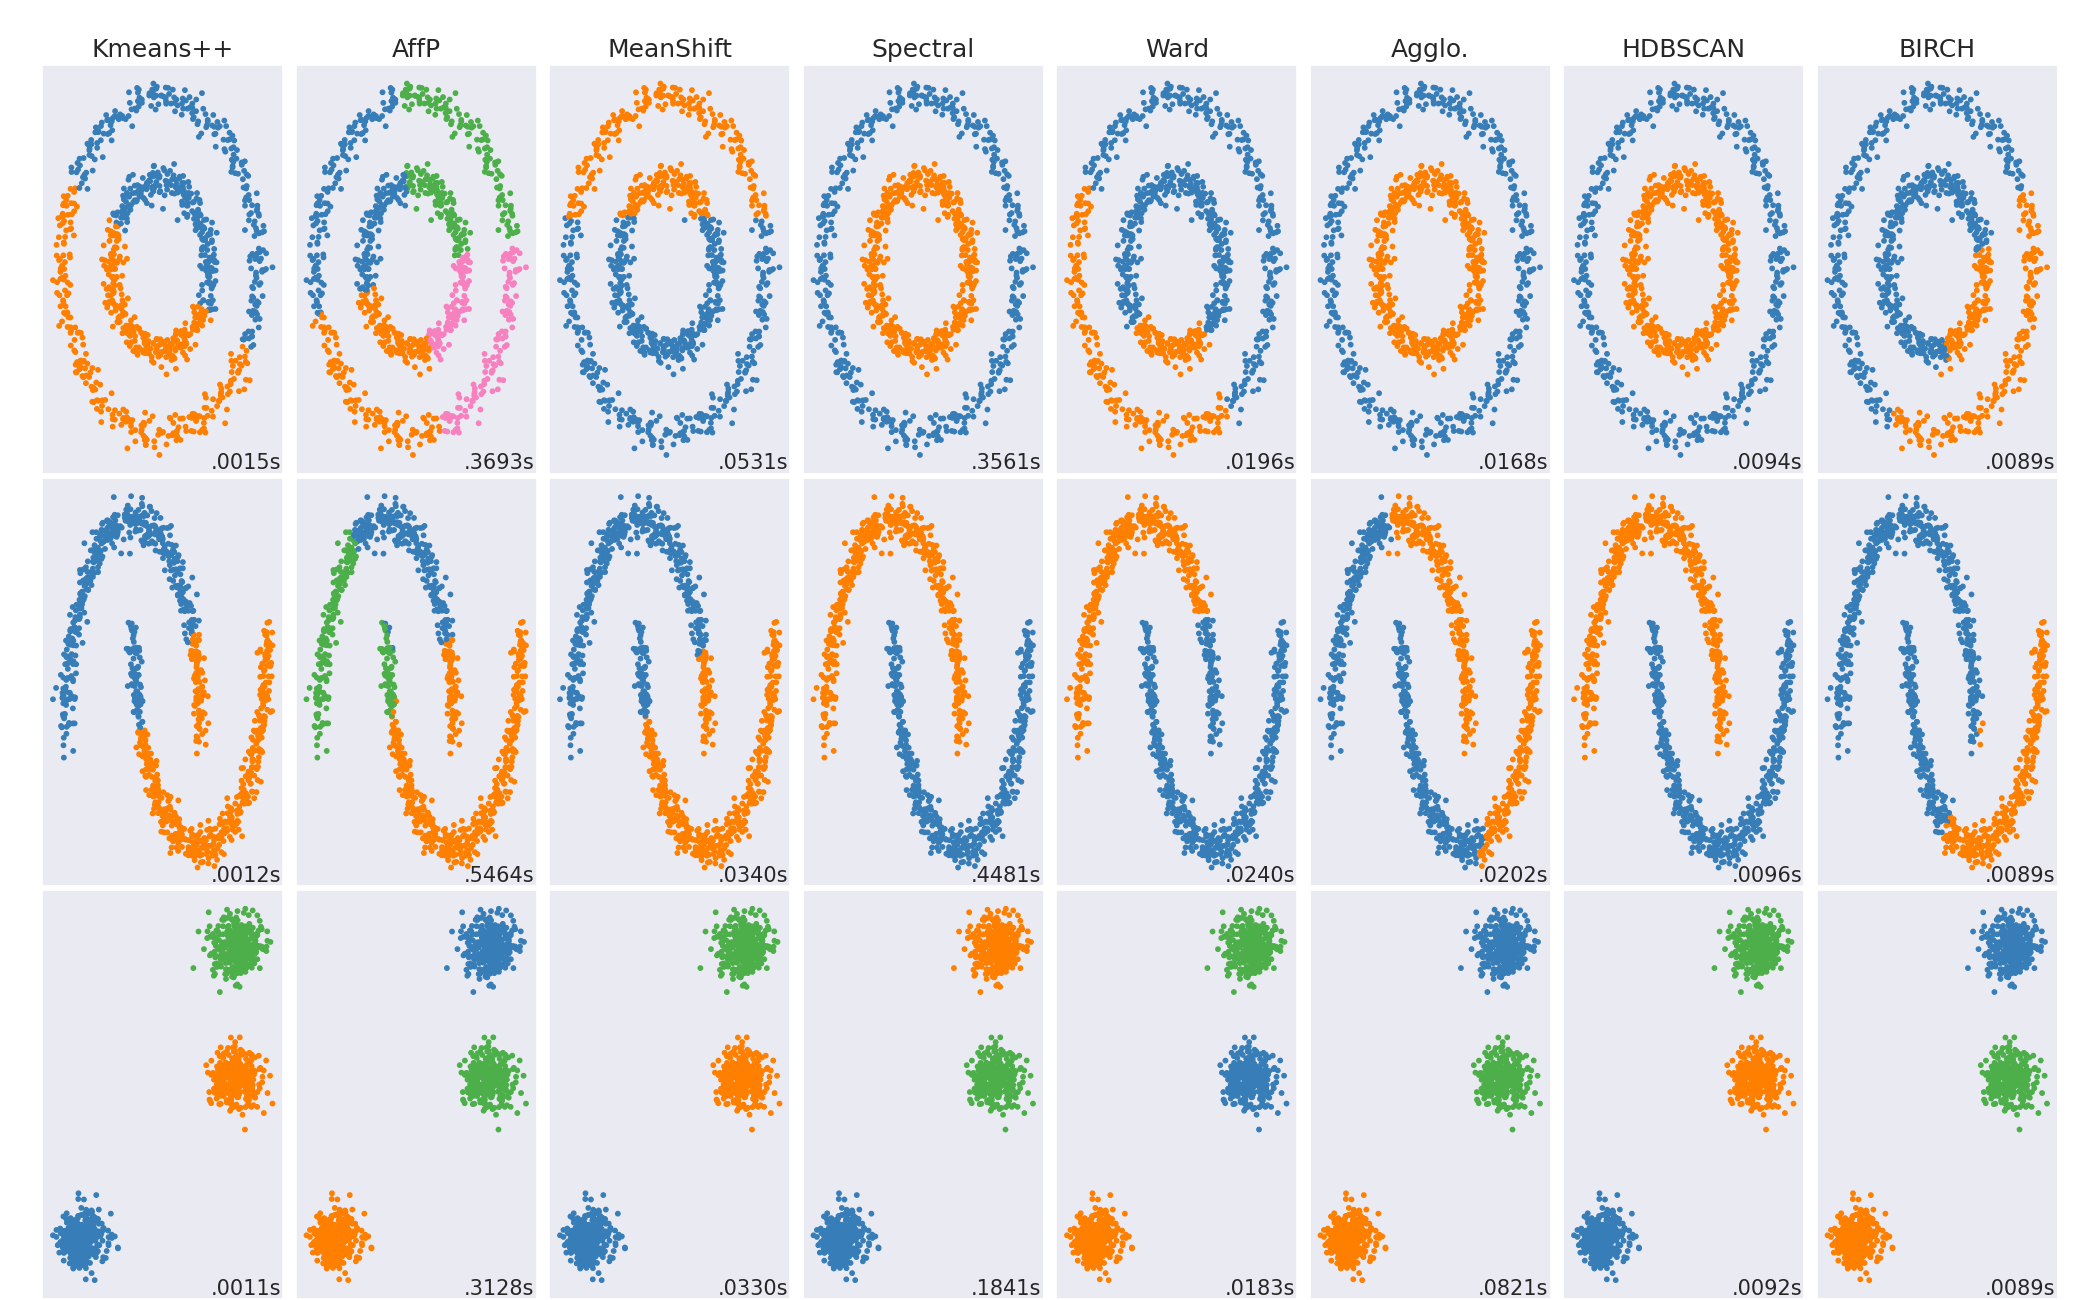
\includegraphics[width=\linewidth]{../clustering_result_1000}
			\captionof{figure}{Time taken for 1000 points}
		\end{minipage}
		\hfill
		\begin{minipage}{.9\linewidth}
			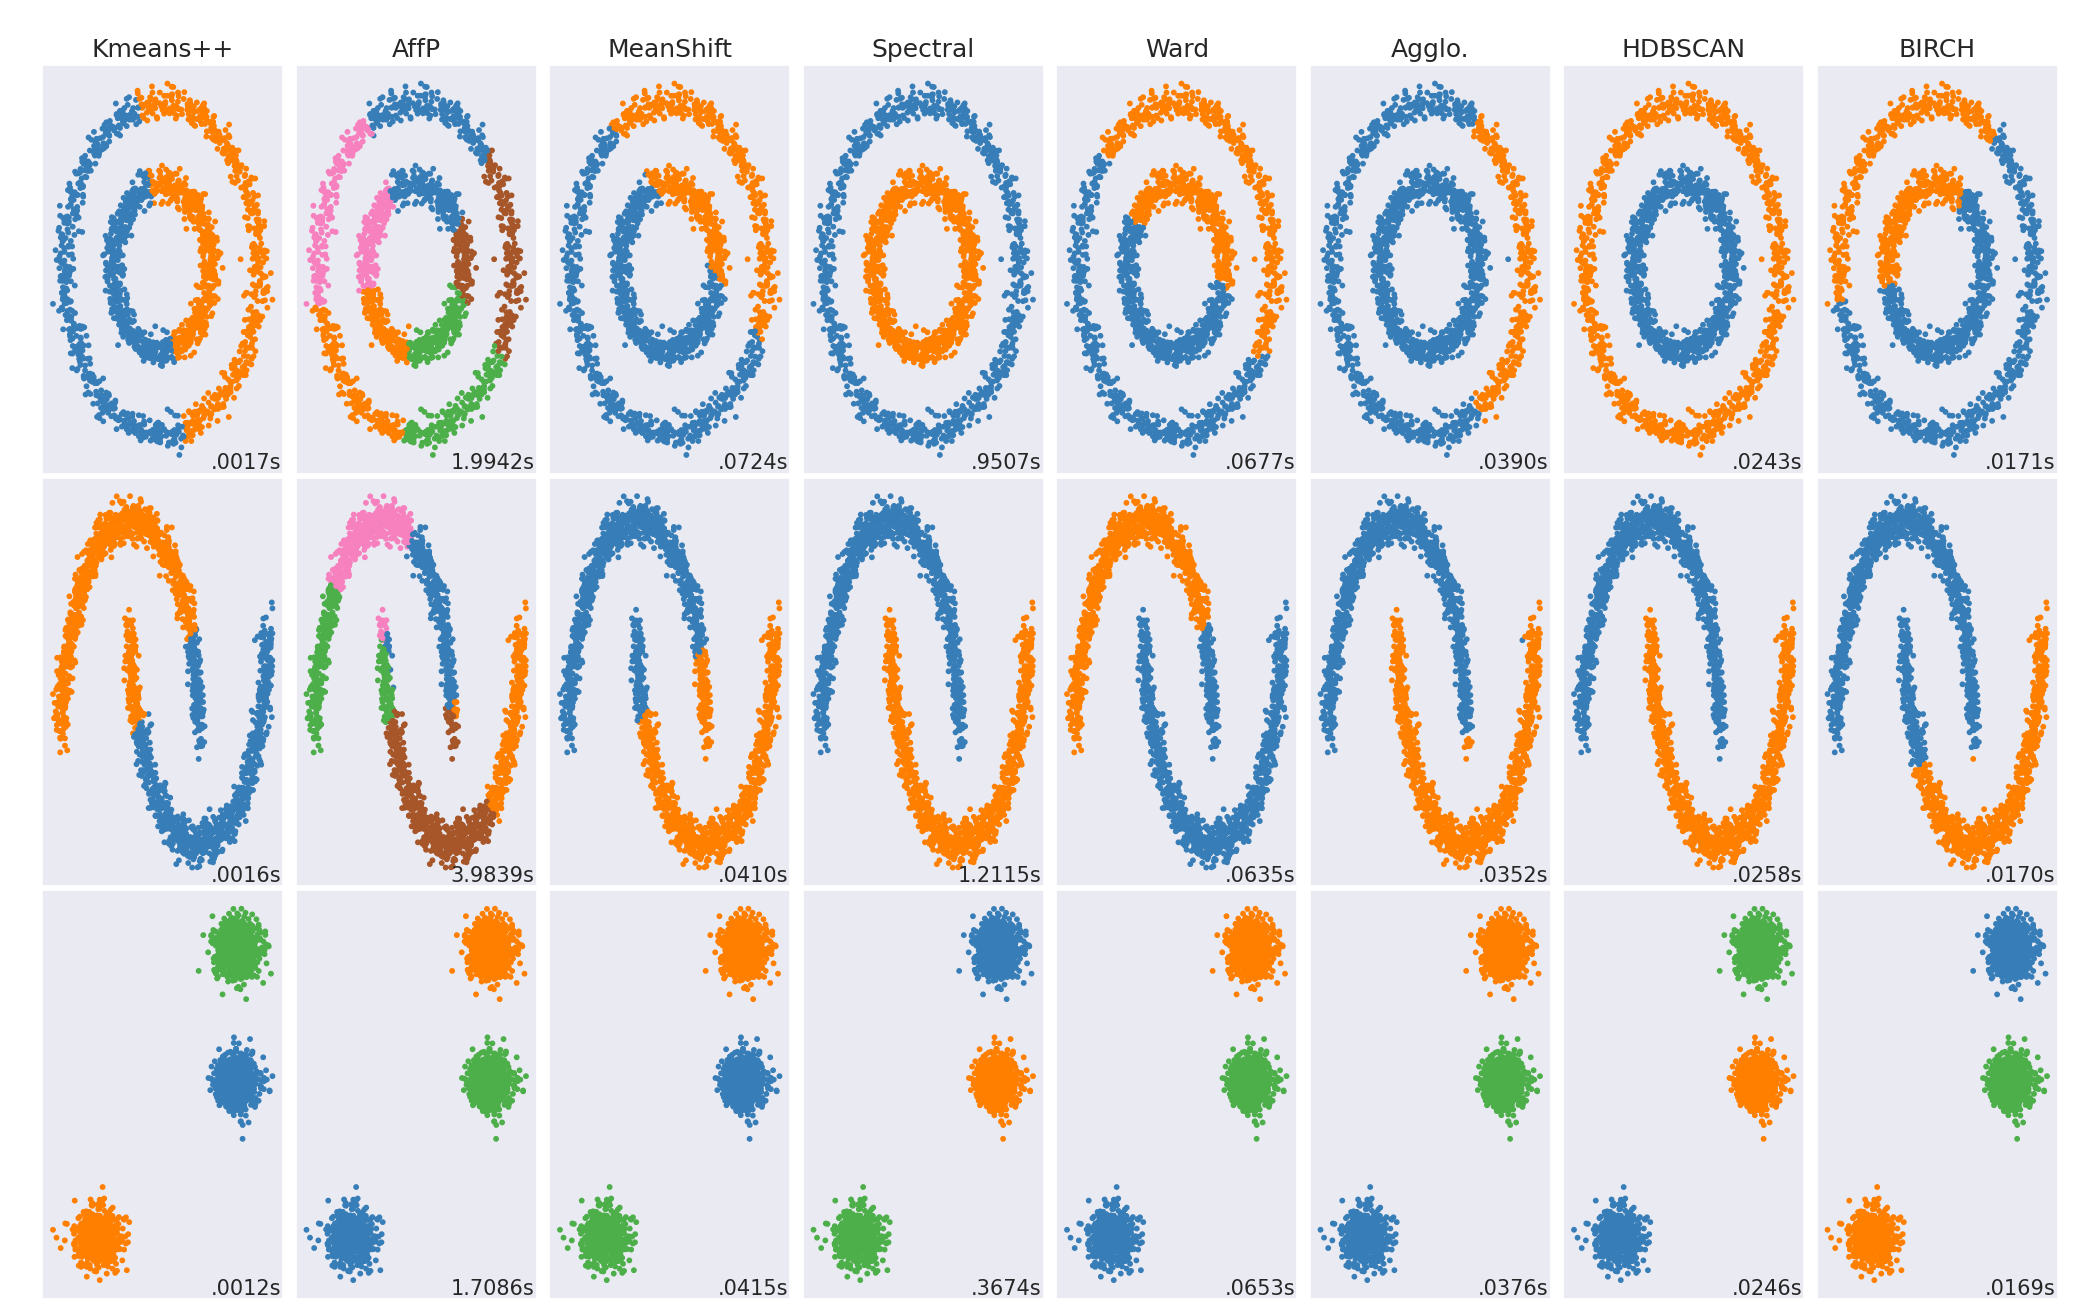
\includegraphics[width=\linewidth]{../clustering_result_2000}
			\captionof{figure}{Time taken for 2000 points}
		\end{minipage}%
	\end{center}

	\begin{center}
		\begin{minipage}{.9\linewidth}
			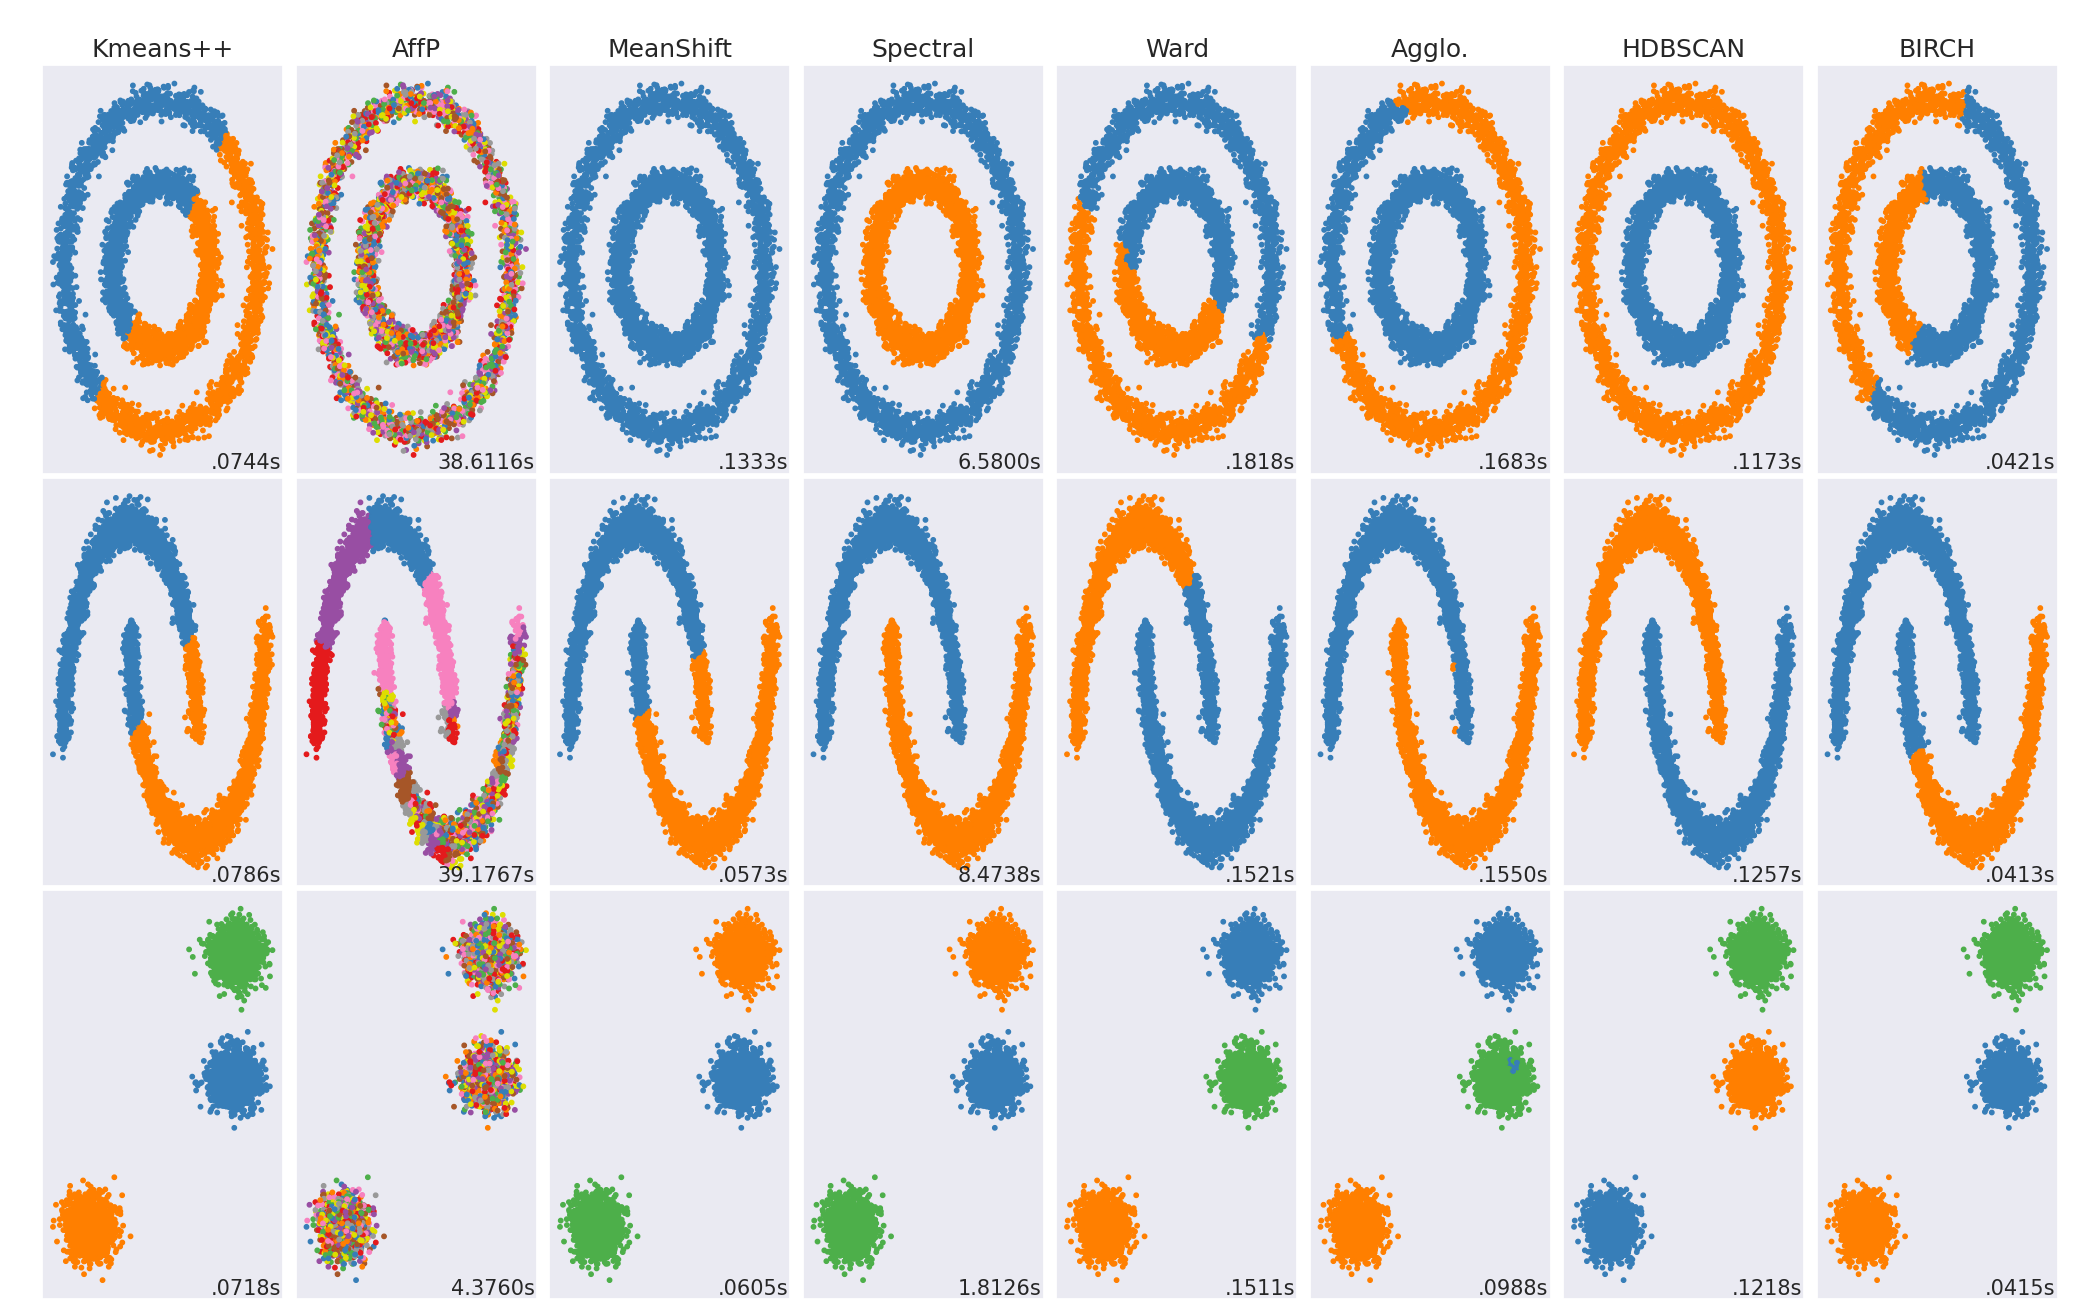
\includegraphics[width=\linewidth]{../clustering_result_5000}
			\captionof{figure}{Time taken for 5000 points}
		\end{minipage}
		\hfill
		\begin{minipage}{.9\linewidth}
			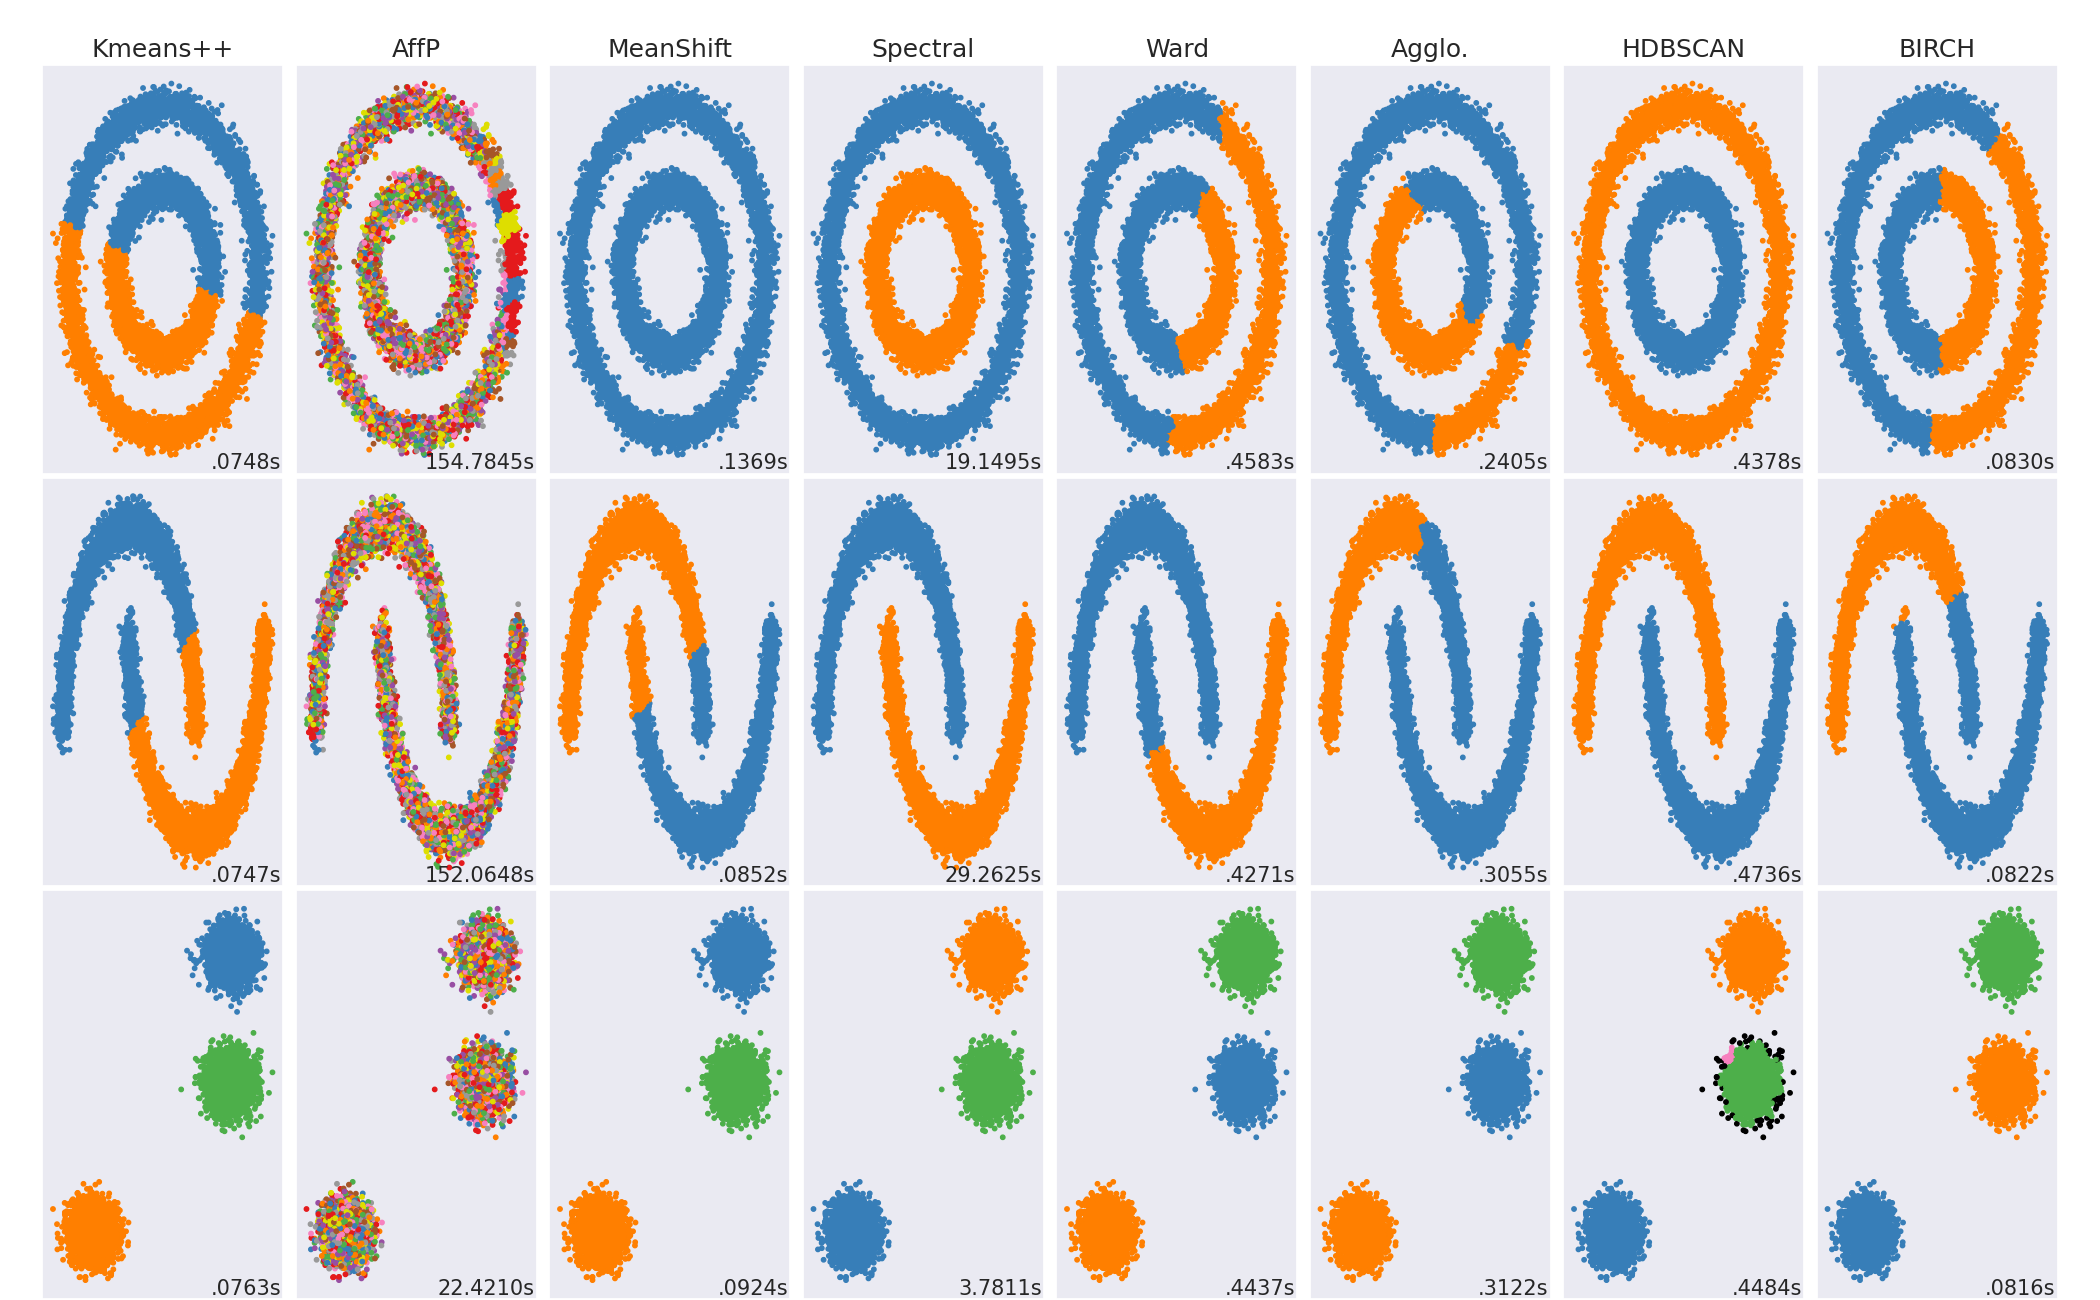
\includegraphics[width=\linewidth]{../clustering_result_10000}
			\captionof{figure}{Time taken for 10000 points}
		\end{minipage}
	\end{center}

	\section{Concerns Regarding \texttt{k-means++} Paper}\label{sec:kmeans++vsorss}
	Given how simple Lloyd's algorithm is, it seems very justified that it is the most popular algorithm for \texttt{k-means}. \textcite{ostrovsky_rabani_schulman_swamy_2012} is a great study on the unusual effectiveness of Lloyd's algorithm. Nowadays most of the times initial centers are chosen with a seeded probability rather than at random. This idea has gained much popularity in recent years. Even in the very well known scientific python package \texttt{scikit-learn} \textcite{pedregosa__et_al_2011}, \texttt{k-means++} initialization is supported by default. And it is no surprise considering the theoretical and experimental results are presented in \textcite{arthur_vassilvitskii_2007}. For example, \textcite{arthur_vassilvitskii_2007} claim \texttt{k-means++} is $\log{k}$ competitive which is a very lucrative result without any doubt. Moreover, they show experimental results that \texttt{k-means++} performs tenfold or even better in most data sets. These are all properties we look for in an ideal algorithm. However, the validity of these results seems to be questionable.
	\subsection{\texttt{k-means++} and \texttt{ORSS}}
	The author remarks that \texttt{k-means++} algorithm is actually a special case of \texttt{ORSS} algorithm. In \texttt{k-means++}, the first center is chosen at random. Then every center is chosen based on the minimum distance of the existing centers from the point in consideration, which \textcite{arthur_vassilvitskii_2007} call $D^2$ \textit{weighting}. Now, \texttt{ORSS} chooses two centers $x,y$ with probability proportional to $\|x-y\|^2$. After choosing those two centers, a new center is added to the set of centers in each iteration until there are $k$ centers, which is done exactly as in \texttt{k-means++}. So, the center adding step is same for both \texttt{k-means++} and \texttt{ORSS}.

	Next, we talk about the first step where \texttt{k-means++} chooses first center at random and \texttt{ORSS} chooses two centers with probability proportional to $\|x-y\|^2$. At this point, we would like to point out that our proposed method of improving \texttt{k-means++} is not actually a novel idea. This was already discussed in \textcite{ostrovsky_rabani_schulman_swamy_2012}. Regretfully, we did not know that at the time because we did not read the full paper back then. It was only after we found out that \texttt{k-means++} results could be wrong, we went through the \texttt{ORSS} paper again. When we read their paper for the second time, we found out that they had already mentioned a result \textcite[Page 4, section 3, Paragraph: Running Time]{ostrovsky_rabani_schulman_swamy_2012} similar to ours in their paper. They say that choosing two centers $x,y$ as in \textcite{ostrovsky_rabani_schulman_swamy_2012} is the same as choosing the first center $c_1$ with probability proportional to $\sum_{y\in X}\|x-y\|^2$ and the second center with probability proportional to $\|y-c_1\|^2$. As we will see in section \ref{sec:motivation} that the first step was exactly our idea of improving \texttt{k-means++}. Despite being a duplicate result, we have decided to discuss our reasoning in this paper because we believe our motivation was different than theirs. As for the second step, again, notice that this is the same as second step in \texttt{k-means++}. In \texttt{k-means++}, after the first center has been chosen randomly, a point $x$ actually gets chosen with probability $\|x-c_1\|^2$. The reason is, there is only one center so the minimum distance is the only distance from $c_1$ to $x$. Therefore, we argue that \textcite{ostrovsky_rabani_schulman_swamy_2012} is an improvement\footnote{To be more precise, this is exactly the improvement that we were trying to suggest} over \texttt{k-means++}.
	\subsection{Accuracy of \texttt{k-means++} Results}
	We will now discuss the other issue at hand. Regarding the accuracy of \texttt{k-means++} results, we have two concerns. One is that the theoretical results may not be correct. And the other is that experimental results might not be correct either. This does not imply that \texttt{k-means++} is a bad algorithm. It still works really well, just that we do not think the results mentioned in the paper are correct.

	First, let us discuss the theoretical concern. In \textcite{arthur_vassilvitskii_2007}, $D(x)$ is assumed to be the minimum of squared distances  from $x$ to the centers $\C$. In \textcite[Lemma $3.3$, section $3$]{arthur_vassilvitskii_2007}, for two distinct point $a,a_0\in A$, the authors use \textit{triangle inequality}\footnote{Triangle inequality states that for any triangle $ABC$, we have $\|AB\|+\|BC\|\geq \|AC\|$. This transforms into $|a|+|b|\geq |a+b|$ for real numbers, consequently $|a|+|x-a|\geq |x|$ holds as well.} for expressing $D(a)^2$ in terms of $D(a_0)$ and $\|a-a_0\|$. Check the statement of \textcite[Lemma $3.3$]{arthur_vassilvitskii_2007}.
		\begin{lemma}
			Let $A$ be an arbitrary cluster in $\C_{opt}$ and let $\C$ be an arbitrary clustering. If we add a random center to $\C$ from $A$, chosen with $D^2$ weighting, then $E[\phi(A)] \leq 8\phi_{opt}(A)$.
		\end{lemma}
	The statement seems a bit vague to us for the reason mentioned below. Therefore, it is possible that we did not fully understand what they meant in this lemma. However, based on our interpretation, this lemma is wrong.

	They claim in the proof that $D(a_0)\leq D(a)+\|a-a_0\|$. Our concern is whether this is necessarily true or not. First, they take an arbitrary cluster $A$ from the optimal set of centers $\C_{opt}$. Then they choose a point $a_0$ from $A$ with $D^2$ weighting to be added to $\C$, which is an arbitrary clustering. This is the part where our argument lies. Since a center is being added to $\C$ and not $\C_{opt}$, here $D(a)$ is the minimum distance from $a$ to $\C$. If we consider $D(a)=\min(\|a-\C_{opt}\|)$, then the inequality $D(a_0)\leq D(a)+\|a-a_0\|$ holds true. However, in this case $D(a)=\min(\|a-\C\|)$ should be used instead since the center is being added to $\C$. By definition $D(x)$ is the minimum distance from $x$ to the centers in $\C$ and not $\C_{opt}$. Therefore in the inequality, $D(a)$ and $D(a_0)$ are not distances from the same center and hence, it is not directly implied by triangle inequality. Although nitpicking, we would like to mention that the inequality $\dfrac{a^2+b^2}{2} \geq \left(\dfrac{a+b}{2}\right)^2$ is not the \textit{power mean inequality}. This inequality can be derived in many ways, including power mean inequality, but it itself is not the power mean inequality. For reference, power mean inequality (see \textcite{hardy_littlewood_polya_1934}) states that for any $r\leq s$ and $n$ real numbers $a_1,\cdots,a_n$,
		\begin{align*}
			\left(\dfrac{a_1^r+a_2^r+\cdots+a_n^r}{n}\right)^{\frac{1}{r}} & \leq \left(\dfrac{a_1^s+a_2^s+\cdots+a_n^s}{n}\right)^{\frac{1}{s}}
		\end{align*}
	Since we tried to improve \texttt{k-means++}, obviously we made our own implementations of the algorithm and checked the results against the ones shown in the paper. Our results conflict with some results shown in \texttt{k-means++} paper \textcite{arthur_vassilvitskii_2007}. For this reason, we ran clustering on the same data set (cloud data set) using \texttt{k-means} package from \texttt{scikit-learn} library \textcite{pedregosa__et_al_2011}. We found out that our implementations achieve similar inertia to the one in \texttt{scikit-learn}. On the other hand, results shown in \texttt{k-means++} paper differ from both our and \texttt{scikit-learn} results. At first, we thought this might be due to normalization or standardization. However, even after using both \texttt{min max} and \texttt{standard} normalization (also known as $z$-score), we found out that \texttt{k-means++} results do not match with ours. For cloud data set, both our and \texttt{scikit-learn} implementations have similar inertia values. The results are shown in tables \ref{tbl:cloud_minmaxscaler} (min-max scalar used to process data), \ref{tbl:cloud_no_preprocess} (no pre-processing) and \ref{tbl:cloud_standardscaler} (standard scalar pre-processing). But \texttt{k-means++} results \textcite[Table $3$]{arthur_vassilvitskii_2007} do not match with ours. We confirmed that our data set consisted of $1024$ rows and had dimension $10$. Moreover, we obtained the data set from UC-Irvine Machine Learning Repository which is the same source stated in \textcite[Section $6.1$]{arthur_vassilvitskii_2007}.

	We also tried collecting every data set that was used in \texttt{k-means++} paper but we managed to get only the cloud data set. We could not find the other real world data set \textit{Intrusion} either. There were some similar data sets but they matched neither the number of data points (494019) nor the dimension (35). Therefore, cloud data set was our primary source of comparison. We would like to mention that in a footnote \textcite[Section $6$, page $8$]{arthur_vassilvitskii_2007} mentioned a url that contained full test suite. However, the site seems to be no longer accessible even though the parent sites are. Therefore, we could neither retrieve the original data sets used in their paper nor check\footnote{The author contacted the authors of \texttt{kmeans++} in order to clarify whether it is a misunderstanding on the author's part or a calculation error on their end; however, did not receive any reply.} their implementation.
	\section{Initialization Methods}
	For a set of points $S$ and a point $x$, we use $\min(\|x-S\|)$ to denote the minimum of distances from $x$ to the points of $S$ that is $\min(\| x-S\|)=\min_{a\in S}(\| x-a\|)$. Set $D(\x)=\min(\|\x-\C\|)$ for a point $x$ and a set of centers $\C$. Let us denote the centroid of $S$ by $\mu_S$ that is $\mu_S=\dfrac{1}{|S|}\sum_{x\in S}x$.
	\subsection{First center for \texttt{k-means++}}\label{sec:first_center}
	In \texttt{k-means++} algorithm, the first center is chosen uniformly at random. However, not all points have the same contribution to inertia. We choose $x$ as a first center in a way that is equivalent to the variance explained by $x$.
	\begin{enumerate}[i]
		\item Choose $\x$ with probability $\dfrac{\|\x-\mu_{\X}\|^2}{\sum_{\x\in\X}\|\x-\mu_{\X}\|^2}$. Set $\C_1=\{\x\}$.\label{step:first_center}
		\item Repeat the remaining steps in \texttt{k-means++} \cite[Section $2.2$, Page $3$]{arthur_vassilvitskii_2007}.
	\end{enumerate}
	\subsection{Centroid of Centers Based Seeding}
	We want to choose $x$ with probability proportional to squared distance from centroid of the cluster centers. Our motivation for doing so is the following. In \texttt{k-means++}, probability is considered proportional to squared minimum distance from the centers. Therefore, the larger this minimum squared distance is, the higher the probability is for $x$ to be chosen as a center. So, in a sense this can be thought of maximizing the minimum squared distance from the centers to the point in consideration. We intend to check the case where we choose the probability proportional to the total sum of squared distances rather than just the minimum one. As we will show later, sum of all squared distances from centers to the point in discussion is dependent on the distance from centroid of those cluster centers to that point.
		\begin{enumerate}[i]
			\item Choose a point $\x$ as stated in step \eqref{step:first_center} of section \eqref{sec:first_center}. Set $\C_1=\{\x\}$.
			\item For an already existing set of $i$ centers $\mathcal{C}_i=\{c_1,\cdots,c_i\}$, choose a new center $\x\in\X$ with probability proportional to $\|\x-\mu_{\C_i}\|^2$.\label{step:coc_center}
			\item Repeat step \eqref{step:coc_center} until $i=k$.
			\item For each $1\leq i\leq k$, set $\C_i=\{\x\in\X:\|\x-c_i\|=\min(\x-\C)\}$.\label{step:coc_cluster}
			\item Set $c_i=\mu_{\C_i}$.\label{step:coc_update}
			\item Repeat \eqref{step:coc_cluster} and \eqref{step:coc_update} until convergence is reached.
		\end{enumerate}
	\section{\texttt{k-means++} Improvement}\label{sec:motivation}
	In this section, we discuss the motivation behind our idea of improving \texttt{k-means++}.
	Consider a set of $n$ points $\X$ and that the probability of $x\in\X$ being chosen as a center as $p(x)$. Following the definition of variance, for a set of points $S$, we define
		\begin{align}
			\sigma^2(S) & = \dfrac{\sum_{x\in S} \|x-\mu_{S}\|^2}{|S|}\nonumber\\
			\sum_{x\in S}\|x-\mu_{S}\|^2 & = |S|\sigma^2\label{eqn:1}
		\end{align}
	For any arbitrary point $a$ and $\mu$ as the centroid of $\X$,
		\begin{align}
			\sum_{\x\in\X}\|\x-a\|^2
				  & = \sum_{\x\in\X}\|\x-\mu+\mu-a\|^2\nonumber\\
				  & = \sum_{\x\in\X}\left(\|\x-\mu\|^2+2\langle\x-\mu,\mu-a\rangle+\|\mu-a\|^2\right)\nonumber\\
				  & = \sum_{\x\in\X}\|\x-\mu\|^2+2\left\langle\sum_{\x\in\X}\x-n\mu,\mu-a\right\rangle+n\|\mu-a\|^2\nonumber\\
				  & = n\sigma^2+2\langle n\mu-n\mu,\mu-a\rangle+n\|\mu-a\|^2\nonumber\\
				  & = n(\sigma^2+\|\mu-a\|^2)\label{eqn:2}
		\end{align}
	Here $\langle a,b\rangle$ is the dot product of vectors $a$ and $b$. Using equation \eqref{eqn:2}, we have the following.
		\begin{align}
			\sum_{\x\in\X}\sum_{\y\in\X}\|\x-\y\|^2
				& = \sum_{\x\in\X}n(\sigma^2+\|\mu-\x\|^2)\nonumber\\
				& = n(n\sigma^2+\sum_{\x\in\X}\|\mu-\x\|^2)\nonumber\\
				& = n(n\sigma^2+n\sigma^2)\nonumber\\
				& = 2n^2\sigma^2\label{eqn:3}
		\end{align}
	Using equation \eqref{eqn:3}, the probability becomes
		\begin{align*}
			p(x) & = \dfrac{\sum_{\y\in\X}\|\x-\y\|^2}{\sum_{\y\in\X}\sum_{\x'\in\X}\|\x'-\y\|^2}\\
				 & = \dfrac{n(\sigma^2+\|\mu-\x\|^2)}{2n^2\sigma^2}\\
				 & = \dfrac{\sigma^2+\|\mu-\x\|^2}{2n\sigma^2}\\
				 & = \dfrac{1}{2n}+\dfrac{\|\mu-\x\|^2}{2n\sigma^2}
		\end{align*}
	However, to make things smoother, one can also choose to use the following as the probability of $x$ being chosen as the first center.
		\begin{align*}
			p(x) & = \dfrac{\|\mu-\x\|^2}{n\sigma^2}
		\end{align*}
	Notice that the variance of $S$ is in the denominator. We can think of $p(x)$ as if it is the amount of variance explained by $x$. Also, this version of $p(x)$ is computationally much cheaper than $\sum_{\y\in\X}\|\x-\y\|^2$. Therefore, we considered $p(x)$ proportional to $\|x-\mu\|^2$ for choosing $x$ as the first center in our experiments.
	\section{An Upper Bound on Inertia}
	%Since the algorithms in discussion are probabilistic, we should look at the expected value of inertia. For a set of points $\X$ and a set of centers $\C$, we denote the inertia by $\I_\C(\X)$. %For the optimal set of cluster centers $\C_{opt}$, we denote the corresponding inertia by $\I_{opt}(\X)$.
		%align*}
	For the minimum distance from $D(x)$ from $x$ to the set of points $\C$,
		\begin{align*}
			D(x)^2 & \leq \dfrac{1}{k}\sum_{c\in \C}\|x-c\|^2\\
					& = \dfrac{1}{k}\left(k\|x-\mu_{\C}\|^2+\sum_{c\in\C}\|\mu_{\C}-c\|^2\right)\\
					& = \|x-\mu_{\C}\|^2+\dfrac{1}{k}\sum_{c\in\C}\|\mu_{\C}-c\|^2
		\end{align*}
	Thus, we can write inertia as
		\begin{align*}
			\cal I & = \sum_{x\in S}\min_{c\in C}\|x-c\|^2\\
			D(x)^2 & = \min_{c\in C}\|x-c\|^2\\
			D(x)^2 & \leq \|x-\mu_{C}\|^2+\dfrac{1}{k}\sum_{c\in C}\|\mu_{C}-c\|^2\\
			\cal I & \leq \sum_{x\in S}\left(\|x-\mu_C\|^2+\dfrac1k\cal I_C\right)\\
			& = \sum_{x\in S}\|x-\mu_C\|^2+\dfrac nk\cal I_C\\
			& = \sum_{x\in S}\|x-\mu\|^2+n\|\mu-\mu_C\|^2+\dfrac nk\cal I_C
		\end{align*}
	This holds for any seeding technique. Thus, we get the following.
		\begin{theorem}
			If $S$ is a set of $n$ points and $C$ is a set of $k$ centers, we have
				\begin{align*}
					\I(S) & \leq n(\sigma^2+\|\mu_S-\mu_C\|^2)+\dfrac{n}{k}\I_{opt}(C)
				\end{align*}
			regardless of what seeding method is used.
		\end{theorem}
	\section{Experiment Setup}
	We ensure that all algorithms are run under the same conditions. All of them share the same environment and no special optimizations were made for any particular algorithm. Only CPU was used to determine the values we are interested in and no parallelism mechanism was in place for speeding up the process. This way, we can get an idea about the raw performances of the algorithms involved. Here is the list of data sets used.
		\begin{enumerate}[i]
			\item Boston housing data set
			\item Wine quality testing data set
			\item Mall customers data set
			\item Airlines cluster data set
			\item Cloud data set
			\item Two moons data set
			\item Boston schools data set
			\item Old faithful geyser data set
			\item Iris data set
		\end{enumerate}
	\textcite{milligan_cooper_1988} shows that using $z$-score to standardize the data is not favorable for clustering because it loses between-cluster variation. Therefore, we did not use any sort of standardization or normalization lest it should lose variance or become prone to bias. Instead, we have used PCA to remove linear dependency among variables.

	While experimenting on such algorithms, it is of utmost importance to run the same experiment more than once under the same parameters and conditions. We ran each experiment a total of $20$ times. The average and minimum values of inertia, CPU time taken are reported in the result section.
	\section{Results}\label{sec:results}
	We have shown the results for $k\in\{5,10,25\}$ clusters in tables \ref{tbl:airlines5} to \ref{tbl:Wine25}. As expected, default \texttt{k-means} is usually the fastest algorithm but also the worst in terms of optimizing inertia.

	The comparison of inertia for \texttt{k-means++} seeding is showed in tables \ref{tbl:cloud_no_preprocess}, \ref{tbl:cloud_standardscaler}, \ref{tbl:cloud_minmaxscaler}. We can check the results against \textcite[Table $3$]{arthur_vassilvitskii_2007}. See that even though we used both standard and min-max scaled data, their inertia values do not match with ours for any of the number of clusters in $\{10,25,50\}$. Since both our and \texttt{scikit-learn} implementations achieve similar inertia values, we believe our coding is correct. Also, since the cloud data set we used had exactly the number of dimension and rows as in \textcite{arthur_vassilvitskii_2007}, we believe that this is also the correct data set. \footnote{The code and dataset are available at a Github repository which can be made available upon request.}
		\begin{table}[p]
			\begin{center}
				\begin{tabular}{|l|l|l|l|l|l|l|}
					\hline
					Initialization & Avg. In. & Min. In. & Avg. T & Min. T & Avg. It. & Min. It.\\\hline
					\texttt{random} & 5788610179951.84 & 5788610179951.84 & 1.68 & 1.35 & 34.15 & 28.0\\\hline
					\texttt{k-means++} & 5895771708319.71 & 5724390573955.8 & 1.34 & 0.63 & 25.15 & 10.0\\\hline
					\texttt{orss} & 5833118291028.73 & 5724390573955.8 & 1.29 & 0.68 & 23.9 & 11.0\\\hline
					\texttt{coc} & 5788610179951.84 & 5788610179951.84 & 1.51 & 0.92 & 30.2 & 18.0\\\hline
				\end{tabular}
				\caption{Results on airlines data set, 5 clusters}
				\label{tbl:airlines5}
			\end{center}
		\end{table}

		\begin{table}[p]
			\begin{center}
				\begin{tabular}{|l|l|l|l|l|l|l|}
					\hline
					Initialization & Avg. In. & Min. In. & Avg. T & Min. T & Avg. It. & Min. It.\\\hline
					\texttt{random} & 2812654.07 & 1475549.48 & 0.08 & 0.03 & 10.45 & 3.0\\\hline
					\texttt{k-means++} & 1572564.77 & 1475549.48 & 0.07 & 0.05 & 7.25 & 3.0\\\hline
					\texttt{orss} & 1547677.65 & 1475549.48 & 0.07 & 0.05 & 6.7 & 3.0\\\hline
					\texttt{coc} & 1812654.49 & 1475612.32 & 0.07 & 0.04 & 8.15 & 4.0\\\hline
				\end{tabular}
				\caption{Results on boston data set, 5 clusters}
				\label{tbl:boston5}
			\end{center}
		\end{table}

		\begin{table}[p]
			\begin{center}
				\begin{tabular}{|l|l|l|l|l|l|l|}
					\hline
					Initialization & Avg. In. & Min. In. & Avg. T & Min. T & Avg. It. & Min. It.\\\hline
					\texttt{random} & 17740103.9 & 17700010.65 & 0.52 & 0.12 & 36.85 & 7.0\\\hline
					\texttt{k-means++} & 17821421.19 & 17700010.65 & 0.32 & 0.11 & 20.05 & 4.0\\\hline
					\texttt{orss} & 17980303.16 & 17699943.72 & 0.28 & 0.11 & 17.2 & 4.0\\\hline
					\texttt{coc} & 17740103.9 & 17700010.65 & 0.51 & 0.2 & 35.75 & 13.0\\\hline
				\end{tabular}
				\caption{Results on cloud data set, 5 clusters}
				\label{tbl:cloud5}
			\end{center}
		\end{table}

		\begin{table}[p]
			\begin{center}
				\begin{tabular}{|l|l|l|l|l|l|l|}
					\hline
					Initialization & Avg. In. & Min. In. & Avg. T & Min. T & Avg. It. & Min. It.\\\hline
					\texttt{random} & 59.34 & 50.33 & 0.02 & 0.01 & 8.25 & 4.0\\\hline
					\texttt{k-means++} & 58.48 & 50.28 & 0.02 & 0.01 & 5.1 & 1.0\\\hline
					\texttt{orss} & 56.69 & 50.28 & 0.02 & 0.01 & 4.65 & 2.0\\\hline
					\texttt{coc} & 62.37 & 50.36 & 0.02 & 0.01 & 7.25 & 3.0\\\hline
				\end{tabular}
				\caption{Results on iris data set, 5 clusters}
				\label{tbl:iris5}
			\end{center}
		\end{table}

		\begin{table}[p]
			\begin{center}
				\begin{tabular}{|l|l|l|l|l|l|l|}
					\hline
					Initialization & Avg. In. & Min. In. & Avg. T & Min. T & Avg. It. & Min. It.\\\hline
					\texttt{random} & 84038.0 & 75412.6 & 0.02 & 0.01 & 8.0 & 3.0\\\hline
					\texttt{k-means++} & 82360.19 & 75399.62 & 0.02 & 0.01 & 6.25 & 2.0\\\hline
					\texttt{orss} & 82455.88 & 75399.62 & 0.03 & 0.02 & 6.7 & 3.0\\\hline
					\texttt{coc} & 85772.29 & 75427.71 & 0.03 & 0.01 & 8.4 & 4.0\\\hline
				\end{tabular}
				\caption{Results on mall data set, 5 clusters}
				\label{tbl:mall5}
			\end{center}
		\end{table}

		\begin{table}[p]
			\begin{center}
				\begin{tabular}{|l|l|l|l|l|l|l|}
					\hline
					Initialization & Avg. In. & Min. In. & Avg. T & Min. T & Avg. It. & Min. It.\\\hline
					\texttt{random} & 22.8 & 18.89 & 0.01 & 0.01 & 5.5 & 3.0\\\hline
					\texttt{k-means++} & 20.01 & 18.89 & 0.01 & 0.01 & 4.5 & 2.0\\\hline
					\texttt{orss} & 19.78 & 18.89 & 0.01 & 0.01 & 4.35 & 2.0\\\hline
					\texttt{coc} & 21.98 & 18.91 & 0.01 & 0.01 & 5.05 & 2.0\\\hline
				\end{tabular}
				\caption{Results on moons data set, 5 clusters}
				\label{tbl:moons5}
			\end{center}
		\end{table}

		\begin{table}[p]
			\begin{center}
				\begin{tabular}{|l|l|l|l|l|l|l|}
					\hline
					Initialization & Avg. In. & Min. In. & Avg. T & Min. T & Avg. It. & Min. It.\\\hline
					\texttt{random} & 2106.59 & 2028.44 & 0.03 & 0.01 & 6.85 & 2.0\\\hline
					\texttt{k-means++} & 2162.48 & 2028.44 & 0.03 & 0.02 & 5.05 & 2.0\\\hline
					\texttt{orss} & 2143.76 & 2036.83 & 0.03 & 0.02 & 4.9 & 2.0\\\hline
					\texttt{coc} & 2164.2 & 2028.44 & 0.03 & 0.02 & 5.75 & 3.0\\\hline
				\end{tabular}
				\caption{Results on old data set, 5 clusters}
				\label{tbl:old5}
			\end{center}
		\end{table}

		\begin{table}[p]
			\begin{center}
				\begin{tabular}{|l|l|l|l|l|l|l|}
					\hline
					Initialization & Avg. In. & Min. In. & Avg. T & Min. T & Avg. It. & Min. It.\\\hline
					\texttt{random} & 5911401430.11 & 5733432489.75 & 0.03 & 0.01 & 13.45 & 6.0\\\hline
					\texttt{k-means++} & 6151075153.7 & 5733432489.75 & 0.02 & 0.01 & 9.75 & 3.0\\\hline
					\texttt{orss} & 6037398253.1 & 5734713233.58 & 0.03 & 0.01 & 11.2 & 4.0\\\hline
					\texttt{coc} & 6116023527.58 & 5733432489.75 & 0.02 & 0.01 & 9.6 & 3.0\\\hline
				\end{tabular}
				\caption{Results on schools data set, 5 clusters}
				\label{tbl:schools5}
			\end{center}
		\end{table}

		\begin{table}[p]
			\begin{center}
				\begin{tabular}{|l|l|l|l|l|l|l|}
					\hline
					Initialization & Avg. In. & Min. In. & Avg. T & Min. T & Avg. It. & Min. It.\\\hline
					\texttt{random} & 1005296.55 & 916424.19 & 0.03 & 0.01 & 10.5 & 4.0\\\hline
					\texttt{k-means++} & 1005490.9 & 916424.19 & 0.02 & 0.02 & 6.25 & 3.0\\\hline
					\texttt{orss} & 981833.05 & 916424.19 & 0.02 & 0.01 & 5.7 & 2.0\\\hline
					\texttt{coc} & 1004998.14 & 916424.19 & 0.02 & 0.01 & 6.95 & 3.0\\\hline
				\end{tabular}
				\caption{Results on Wine data set, 5 clusters}
				\label{tbl:Wine5}
			\end{center}
		\end{table}

		\begin{table}[p]
			\begin{center}
				\begin{tabular}{|l|l|l|l|l|l|l|}
					\hline
					Initialization & Avg. In. & Min. In. & Avg. T & Min. T & Avg. It. & Min. It.\\\hline
					\texttt{random} & 5788610179951.84 & 5788610179951.84 & 1.91 & 1.3 & 35.25 & 23.0\\\hline
					\texttt{k-means++} & 5841017195498.52 & 5724390573955.8 & 1.49 & 0.64 & 26.5 & 10.0\\\hline
					\texttt{orss} & 5920823727383.38 & 5724390573955.8 & 1.36 & 0.68 & 22.1 & 9.0\\\hline
					\texttt{coc} & 5788604697505.78 & 5788500531030.62 & 1.68 & 1.23 & 29.5 & 22.0\\\hline
				\end{tabular}
				\caption{Results on airlines data set, 10 clusters}
				\label{tbl:airlines10}
			\end{center}
		\end{table}

		\begin{table}[p]
			\begin{center}
				\begin{tabular}{|l|l|l|l|l|l|l|}
					\hline
					Initialization & Avg. In. & Min. In. & Avg. T & Min. T & Avg. It. & Min. It.\\\hline
					\texttt{random} & 2717448.59 & 1500209.99 & 0.08 & 0.04 & 9.45 & 4.0\\\hline
					\texttt{k-means++} & 1687335.04 & 1475549.48 & 0.08 & 0.05 & 7.2 & 3.0\\\hline
					\texttt{orss} & 1782584.85 & 1475549.48 & 0.09 & 0.05 & 8.1 & 3.0\\\hline
					\texttt{coc} & 1564391.58 & 1476556.31 & 0.09 & 0.05 & 9.7 & 5.0\\\hline
				\end{tabular}
				\caption{Results on boston data set, 10 clusters}
				\label{tbl:boston10}
			\end{center}
		\end{table}

		\begin{table}[p]
			\begin{center}
				\begin{tabular}{|l|l|l|l|l|l|l|}
					\hline
					Initialization & Avg. In. & Min. In. & Avg. T & Min. T & Avg. It. & Min. It.\\\hline
					\texttt{random} & 17700272.49 & 17700010.65 & 0.56 & 0.18 & 37.65 & 11.0\\\hline
					\texttt{k-means++} & 17941909.09 & 17700010.65 & 0.34 & 0.13 & 19.5 & 5.0\\\hline
					\texttt{orss} & 17941152.22 & 17700010.65 & 0.37 & 0.12 & 22.05 & 4.0\\\hline
					\texttt{coc} & 17780988.12 & 17700010.65 & 0.47 & 0.12 & 30.4 & 6.0\\\hline
				\end{tabular}
				\caption{Results on cloud data set, 10 clusters}
				\label{tbl:cloud10}
			\end{center}
		\end{table}

		\begin{table}[p]
			\begin{center}
				\begin{tabular}{|l|l|l|l|l|l|l|}
					\hline
					Initialization & Avg. In. & Min. In. & Avg. T & Min. T & Avg. It. & Min. It.\\\hline
					\texttt{random} & 58.41 & 50.33 & 0.02 & 0.01 & 6.05 & 2.0\\\hline
					\texttt{k-means++} & 59.14 & 50.28 & 0.02 & 0.01 & 5.8 & 2.0\\\hline
					\texttt{orss} & 56.36 & 50.28 & 0.02 & 0.01 & 4.6 & 2.0\\\hline
					\texttt{coc} & 62.19 & 50.28 & 0.02 & 0.01 & 6.55 & 2.0\\\hline
				\end{tabular}
				\caption{Results on iris data set, 10 clusters}
				\label{tbl:iris10}
			\end{center}
		\end{table}

		\begin{table}[p]
			\begin{center}
				\begin{tabular}{|l|l|l|l|l|l|l|}
					\hline
					Initialization & Avg. In. & Min. In. & Avg. T & Min. T & Avg. It. & Min. It.\\\hline
					\texttt{random} & 84902.83 & 75399.62 & 0.04 & 0.02 & 7.9 & 4.0\\\hline
					\texttt{k-means++} & 81352.0 & 75399.62 & 0.05 & 0.03 & 5.65 & 3.0\\\hline
					\texttt{orss} & 81631.34 & 75399.62 & 0.05 & 0.03 & 8.65 & 3.0\\\hline
					\texttt{coc} & 83759.84 & 75427.71 & 0.04 & 0.02 & 8.4 & 3.0\\\hline
				\end{tabular}
				\caption{Results on mall data set, 10 clusters}
				\label{tbl:mall10}
			\end{center}
		\end{table}

		\begin{table}[p]
			\begin{center}
				\begin{tabular}{|l|l|l|l|l|l|l|}
					\hline
					Initialization & Avg. In. & Min. In. & Avg. T & Min. T & Avg. It. & Min. It.\\\hline
					\texttt{random} & 23.62 & 18.91 & 0.02 & 0.01 & 5.7 & 4.0\\\hline
					\texttt{k-means++} & 20.22 & 18.89 & 0.01 & 0.01 & 4.2 & 1.0\\\hline
					\texttt{orss} & 20.46 & 18.89 & 0.01 & 0.01 & 4.7 & 2.0\\\hline
					\texttt{coc} & 20.4 & 18.89 & 0.01 & 0.01 & 5.5 & 2.0\\\hline
				\end{tabular}
				\caption{Results on moons data set, 10 clusters}
				\label{tbl:moons10}
			\end{center}
		\end{table}

		\begin{table}[p]
			\begin{center}
				\begin{tabular}{|l|l|l|l|l|l|l|}
					\hline
					Initialization & Avg. In. & Min. In. & Avg. T & Min. T & Avg. It. & Min. It.\\\hline
					\texttt{random} & 2186.18 & 2028.44 & 0.04 & 0.01 & 7.1 & 2.0\\\hline
					\texttt{k-means++} & 2222.88 & 2039.55 & 0.04 & 0.02 & 4.7 & 2.0\\\hline
					\texttt{orss} & 2171.94 & 2028.44 & 0.03 & 0.02 & 3.5 & 1.0\\\hline
					\texttt{coc} & 2188.5 & 2028.44 & 0.03 & 0.02 & 5.85 & 2.0\\\hline
				\end{tabular}
				\caption{Results on old data set, 10 clusters}
				\label{tbl:old10}
			\end{center}
		\end{table}

		\begin{table}[p]
			\begin{center}
				\begin{tabular}{|l|l|l|l|l|l|l|}
					\hline
					Initialization & Avg. In. & Min. In. & Avg. T & Min. T & Avg. It. & Min. It.\\\hline
					\texttt{random} & 6036905058.56 & 5729423591.21 & 0.02 & 0.01 & 9.95 & 4.0\\\hline
					\texttt{k-means++} & 6071879236.33 & 5728232615.59 & 0.02 & 0.01 & 7.95 & 2.0\\\hline
					\texttt{orss} & 6152682962.47 & 5729423591.21 & 0.03 & 0.02 & 8.4 & 4.0\\\hline
					\texttt{coc} & 6122042430.59 & 5739498515.77 & 0.03 & 0.01 & 11.85 & 4.0\\\hline
				\end{tabular}
				\caption{Results on schools data set, 10 clusters}
				\label{tbl:schools10}
			\end{center}
		\end{table}

		\begin{table}[p]
			\begin{center}
				\begin{tabular}{|l|l|l|l|l|l|l|}
					\hline
					Initialization & Avg. In. & Min. In. & Avg. T & Min. T & Avg. It. & Min. It.\\\hline
					\texttt{random} & 1010055.91 & 916424.19 & 0.03 & 0.01 & 9.2 & 3.0\\\hline
					\texttt{k-means++} & 990859.67 & 916424.19 & 0.03 & 0.02 & 6.25 & 3.0\\\hline
					\texttt{orss} & 1014711.02 & 916424.19 & 0.03 & 0.02 & 5.95 & 2.0\\\hline
					\texttt{coc} & 1005327.62 & 916424.19 & 0.03 & 0.01 & 7.95 & 3.0\\\hline
				\end{tabular}
				\caption{Results on Wine data set, 10 clusters}
				\label{tbl:Wine10}
			\end{center}
		\end{table}

		\begin{table}[p]
			\begin{center}
				\begin{tabular}{|l|l|l|l|l|l|l|}
					\hline
					Initialization & Avg. In. & Min. In. & Avg. T & Min. T & Avg. It. & Min. It.\\\hline
					\texttt{random} & 1179535.38 & 726875.22 & 0.18 & 0.11 & 13.95 & 7.0\\\hline
					\texttt{k-means++} & 796562.49 & 707943.36 & 0.17 & 0.12 & 8.55 & 4.0\\\hline
					\texttt{orss} & 783434.35 & 708148.86 & 0.19 & 0.12 & 9.85 & 4.0\\\hline
					\texttt{coc} & 836074.29 & 714810.01 & 0.22 & 0.12 & 15.65 & 7.0\\\hline
				\end{tabular}
				\caption{Results on boston data set, 25 clusters}
				\label{tbl:boston25}
			\end{center}
		\end{table}

		\begin{table}[p]
			\begin{center}
				\begin{tabular}{|l|l|l|l|l|l|l|}
					\hline
					Initialization & Avg. In. & Min. In. & Avg. T & Min. T & Avg. It. & Min. It.\\\hline
					\texttt{random} & 7778602.59 & 6286432.16 & 1.13 & 0.39 & 46.5 & 15.0\\\hline
					\texttt{k-means++} & 6175654.25 & 5754925.79 & 0.66 & 0.24 & 21.55 & 4.0\\\hline
					\texttt{orss} & 6313890.31 & 5754925.79 & 0.79 & 0.34 & 27.85 & 7.0\\\hline
					\texttt{coc} & 6684716.64 & 5754925.79 & 1.49 & 0.27 & 64.15 & 10.0\\\hline
				\end{tabular}
				\caption{Results on cloud data set, 25 clusters}
				\label{tbl:cloud25}
			\end{center}
		\end{table}

		\begin{table}[p]
			\begin{center}
				\begin{tabular}{|l|l|l|l|l|l|l|}
					\hline
					Initialization & Avg. In. & Min. In. & Avg. T & Min. T & Avg. It. & Min. It.\\\hline
					\texttt{random} & 31.57 & 27.59 & 0.03 & 0.02 & 6.85 & 4.0\\\hline
					\texttt{k-means++} & 29.41 & 27.29 & 0.04 & 0.03 & 4.75 & 3.0\\\hline
					\texttt{orss} & 30.38 & 26.84 & 0.04 & 0.03 & 5.8 & 3.0\\\hline
					\texttt{coc} & 34.62 & 28.35 & 0.04 & 0.02 & 8.2 & 4.0\\\hline
				\end{tabular}
				\caption{Results on iris data set, 25 clusters}
				\label{tbl:iris25}
			\end{center}
		\end{table}

		\begin{table}[p]
			\begin{center}
				\begin{tabular}{|l|l|l|l|l|l|l|}
					\hline
					Initialization & Avg. In. & Min. In. & Avg. T & Min. T & Avg. It. & Min. It.\\\hline
					\texttt{random} & 43066.3 & 37747.05 & 0.04 & 0.03 & 7.9 & 5.0\\\hline
					\texttt{k-means++} & 40317.7 & 37581.02 & 0.05 & 0.05 & 6.1 & 4.0\\\hline
					\texttt{orss} & 40096.13 & 37819.5 & 0.06 & 0.05 & 6.15 & 4.0\\\hline
					\texttt{coc} & 42233.13 & 39118.08 & 0.05 & 0.03 & 8.15 & 5.0\\\hline
				\end{tabular}
				\caption{Results on mall data set, 25 clusters}
				\label{tbl:mall25}
			\end{center}
		\end{table}

		\begin{table}[p]
			\begin{center}
				\begin{tabular}{|l|l|l|l|l|l|l|}
					\hline
					Initialization & Avg. In. & Min. In. & Avg. T & Min. T & Avg. It. & Min. It.\\\hline
					\texttt{random} & 10.26 & 7.6 & 0.02 & 0.01 & 7.05 & 4.0\\\hline
					\texttt{k-means++} & 9.24 & 8.06 & 0.03 & 0.02 & 5.1 & 3.0\\\hline
					\texttt{orss} & 8.78 & 7.59 & 0.02 & 0.02 & 4.25 & 2.0\\\hline
					\texttt{coc} & 10.57 & 7.58 & 0.02 & 0.01 & 6.85 & 3.0\\\hline
				\end{tabular}
				\caption{Results on moons data set, 25 clusters}
				\label{tbl:moons25}
			\end{center}
		\end{table}

		\begin{table}[p]
			\begin{center}
				\begin{tabular}{|l|l|l|l|l|l|l|}
					\hline
					Initialization & Avg. In. & Min. In. & Avg. T & Min. T & Avg. It. & Min. It.\\\hline
					\texttt{random} & 767.68 & 541.06 & 0.04 & 0.03 & 5.15 & 3.0\\\hline
					\texttt{k-means++} & 599.9 & 545.47 & 0.06 & 0.05 & 3.65 & 2.0\\\hline
					\texttt{orss} & 636.81 & 553.1 & 0.06 & 0.06 & 4.0 & 3.0\\\hline
					\texttt{coc} & 747.26 & 556.26 & 0.05 & 0.03 & 6.05 & 2.0\\\hline
				\end{tabular}
				\caption{Results on old data set, 25 clusters}
				\label{tbl:old25}
			\end{center}
		\end{table}

		\begin{table}[p]
			\begin{center}
				\begin{tabular}{|l|l|l|l|l|l|l|}
					\hline
					Initialization & Avg. In. & Min. In. & Avg. T & Min. T & Avg. It. & Min. It.\\\hline
					\texttt{random} & 2780499617.96 & 2382345958.39 & 0.03 & 0.02 & 7.85 & 3.0\\\hline
					\texttt{k-means++} & 2574515408.9 & 2346464028.7 & 0.04 & 0.02 & 6.1 & 2.0\\\hline
					\texttt{orss} & 2564154859.1 & 2413558849.09 & 0.04 & 0.03 & 7.05 & 3.0\\\hline
					\texttt{coc} & 2870371762.13 & 2436964942.43 & 0.03 & 0.02 & 8.75 & 4.0\\\hline
				\end{tabular}
				\caption{Results on schools data set, 25 clusters}
				\label{tbl:schools25}
			\end{center}
		\end{table}

		\begin{table}[p]
			\begin{center}
				\begin{tabular}{|l|l|l|l|l|l|l|}
					\hline
					Initialization & Avg. In. & Min. In. & Avg. T & Min. T & Avg. It. & Min. It.\\\hline
					\texttt{random} & 341878.83 & 219710.39 & 0.05 & 0.02 & 10.3 & 4.0\\\hline
					\texttt{k-means++} & 249461.66 & 224847.92 & 0.05 & 0.04 & 5.9 & 3.0\\\hline
					\texttt{orss} & 242546.38 & 218112.55 & 0.05 & 0.04 & 7.05 & 4.0\\\hline
					\texttt{coc} & 273645.86 & 234824.73 & 0.08 & 0.04 & 16.2 & 8.0\\\hline
				\end{tabular}
				\caption{Results on Wine data set, 25 clusters}
				\label{tbl:Wine25}
			\end{center}
		\end{table}

		\begin{table}[p]
			\begin{center}
				\begin{tabular}{|l|l|l|}
					\hline
					Clusters & \texttt{sk-learn} Avg. & Our Avg.\\\hline
					5 & 17706689.573774982& 17711385.61029025\\\hline
					10 & 5761674.929143367& 6434641.098051261\\\hline
					25 & 2007444.7098438586& 2255902.212313077\\\hline
					50 & 1099395.4420880969& 1194727.658029051\\\hline
				\end{tabular}
				\caption{\texttt{k-mean++} results on cloud data set}
				\label{tbl:cloud_no_preprocess}
			\end{center}
		\end{table}

		\begin{table}[p]
			\begin{center}
				\begin{tabular}{|l|l|l|}
					\hline
					Clusters & \texttt{sk-learn} Avg. & Our Avg.\\\hline
					5 & 2519.79170884024 & 2519.826060045223\\\hline
					10 & 1521.9262422548954 & 1510.9057079504264\\\hline
					25 & 817.4296830232086 & 833.2041864088023\\\hline
					50 & 519.1784696946825 & 543.6392985861094\\\hline
				\end{tabular}
				\caption{\texttt{k-means++} results on cloud data set (standardized)}
				\label{tbl:cloud_standardscaler}
			\end{center}
		\end{table}

		\begin{table}[p]
			\begin{center}
				\begin{tabular}{|l|l|l|}
					\hline
					Clusters & \texttt{sk-learn} Avg. & Our Avg.\\\hline
					5 & 57.096454766857384 & 57.302792493848216\\\hline
					10 & 32.929845052888986 & 32.93489472987519\\\hline
					25 & 17.941355048689374 & 18.50259622163847\\\hline
					50 & 11.362562342560503 & 11.7818373139353\\\hline
				\end{tabular}
				\caption{\texttt{k-means++} results on cloud data set (scaled)}
				\label{tbl:cloud_minmaxscaler}
			\end{center}
		\end{table}
	\clearpage
	\section{Conclusion}
	We presented our arguments about \texttt{k-means++} results and discussed different seeding methods to improve \texttt{k-means} algorithms. Then we talked about different seeding techniques of center initialization and proved an upper bound of inertia. Finally, we showed comparison of seeding methods on $9$ data sets for different number of clusters. Our observation is that \texttt{ORSS} is the most stable algorithm where both \texttt{k-means++} and \texttt{coc} often produce results on the extreme side. For a future improvement, a crucial idea could be to develop a deterministic method of seeding initial centers which would not only eliminate the uncertainty factor from KMeans algorithm but also provide better insights into the structure of the data.
	\paragraph{Ethical Conduct}
	As far as the author(s) is (are) concerned, this paper is not being considered for publication anywhere else nor does it break any ethical guidelines the author(s) can think of. No result is fabricated and code/data can be made available upon request.
	\printbibliography
\end{document}